\documentclass[../main]{subfiles}
\begin{document}

\graphicspath{{../figures/}}




\section{序論}

\begin{figure}[tb]
  \centering
  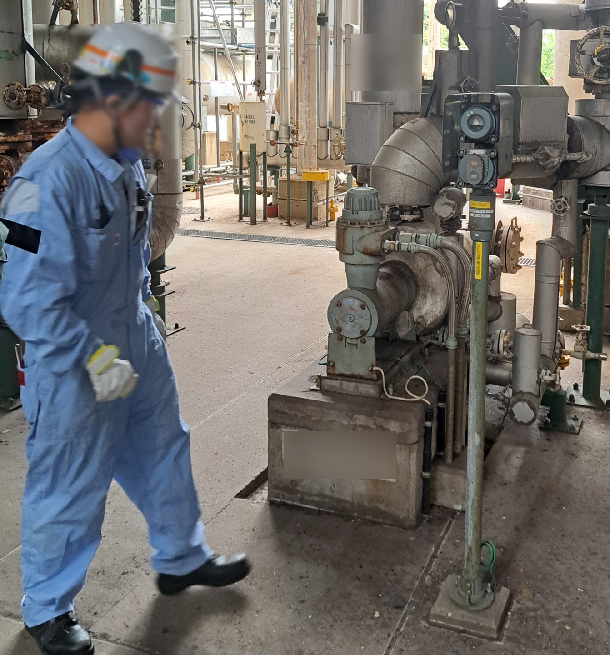
\includegraphics[keepaspectratio, width=0.8\linewidth]{../figures/cyclic_inspection.pdf}
  \caption{石油精製プラント内におけるポンプを対象とした点検の様子}
  \label{fig:cyclic_inspection}
\end{figure}

石油精製プラント内では,機器の老朽化や予期せぬ不調を原因とする様々な異常が存在し,
ベアリングやポンプなどの回転機器が対象の場合は,それらから発せられる音を基に異常の有無を判別する.




従来それらの音による異常の検知は点検員による巡回点検によって行われているが,
人手による巡回点検には,高齢化による熟練点検員の不足や,非熟練点検員による見落としの発生といった問題があげられる.
これらの理由から石油精製プラント内における音響点検を自動化することが求められている.


プラント内における音響点検の自動化には,固定点マイクを複数用いた手法と,移動ロボットにマイクを搭載する手法が考えられる.
固定点マイクを複数用いる場合の課題として,点検箇所の面積が広いため,必要なセンサ数が増加してしまう点,
また,点検対象の危機が密集しており,異常音の発生源を特定することが困難である点が挙げられる.
これらの理由から,石油プラントのような広大かつ機器が密集している環境下では移動ロボットを用いた音響点検が有効であると考えられる.

異常データを異常検知モデルの学習に用いる,教師あり学習の手法を採用している研究にWang~\cite{wang2022}らやNilanon~\cite{Nilanon2016}らの研究がある.
異常データが既知であれば,異常データとのマッチング度合から異常箇所の座標を特定することが可能であるが,多岐にわたる異常データの収集は困難であるという課題が存在する.


また,Fujita~\cite{fujita2023}らは,移動ロボットの経路を区間に分割し,区間ごとに異なる異常検知モデルを学習し,運用時は自己位置に対応する異常検知モデルを選択する手法を提案している.
この手法は,異常データを用いずに異常検知モデルを学習することが可能であるが,区間の異常の有無を判別するものであり,石油プラントのような音響点検の対象となる機器が密集している環境では,
区間内における異常音の発生源となる機器を特定することが困難である.

そのため,本研究では異常音の教師データが不要で異常音源の座標を推定可能な,移動ロボットによる異常音検知手法を目指す.


\end{document}
